\usetikzlibrary{plotmarks}

\begin{figure}[H]
\centering
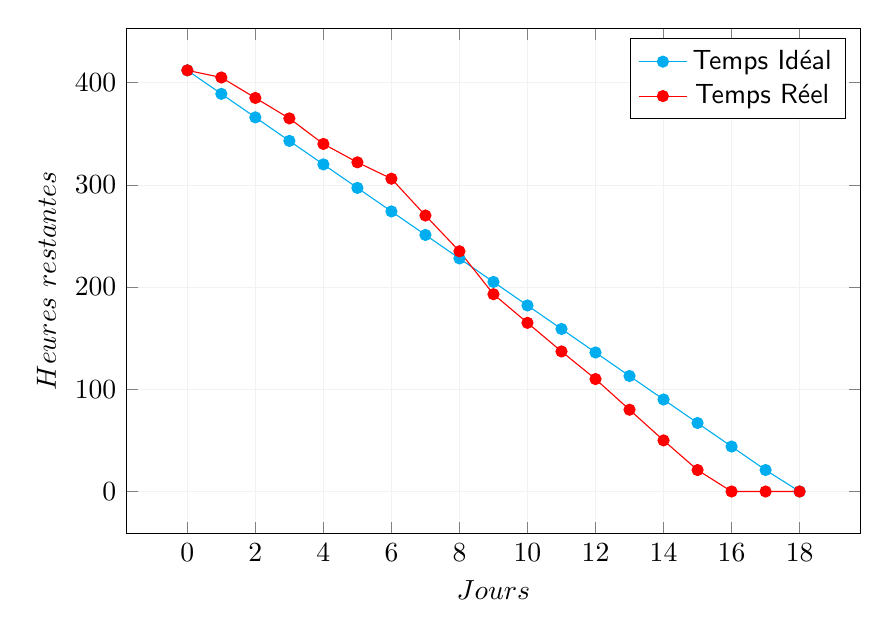
\begin{tikzpicture}[y=.2cm, x=.7cm,font=\sffamily]
\begin{axis}[
xlabel=$Jours$,
ylabel=$Heures\ restantes$,
grid=both,
grid style={line width=.1pt, draw=gray!10},
width=0.9\textwidth,
height=8cm,
%major grid style={line width=.2pt,draw=gray!50},
]
      \addplot[mark=*,cyan] plot coordinates {%
(0, 412)
(1, 389)
(2, 366)
(3, 343)
(4, 320)
(5, 297)
(6, 274)
(7, 251)
(8, 228)
(9, 205)
(10, 182)
(11, 159)
(12, 136)
(13, 113)
(14, 90)
(15, 67)
(16, 44)
(17, 21)
(18, 0)
    };
    \addlegendentry{Temps Idéal}

    \addplot[mark=*,red] plot coordinates {%
        (0, 412)
        (1, 405)
        (2, 385)
        (3, 365)
        (4, 340)
        (5, 322)
        (6, 306)
        (7, 270)
        (8, 235)
        (9, 193)
        (10, 165)
        (11, 137)
        (12, 110)
        (13, 80)
        (14, 50)
        (15, 21)
        (16, 0)
        (17, 0)
        (18, 0)
    };
    \addlegendentry{Temps Réel}
\end{axis}
\end{tikzpicture}
\caption{Graphique d'avancement - Itération 1}
\label{fig:sprint1-burndown}
\end{figure}
